For high-order matrix-free BDDC, we decompose the domain $\Omega$ into a series of subdomains $\Omega^e$ given by the individual elements, and we utilize four non-exclusive spaces on each subdomain.
Figure \ref{fig:bddc_mesh_not_decomposed} shows a global mesh before decomposition, consisting of four quadratic elements in two dimensions in this case.

The interface between subdomains is given by $\Gamma = \bigcup \partial \Omega^e \backslash \partial \Omega$, and the interface of subdomain $\Omega^e$ is given by $\Gamma^e = \delta \Omega^e \bigcap \Gamma$.
The interior of each subdomain, $\text{I}$, is given by the remaining degrees of freedom on the element.
In Figure \ref{fig:bddc_mesh_interface}, the interface degrees of freedom, $\Gamma$, for each subdomain have been highlighted and the interior $\text{I}$ is given by the remainder of each subdomain.

\begin{figure}[!ht]
  \centering
  \subfloat[Global Problem Mesh]{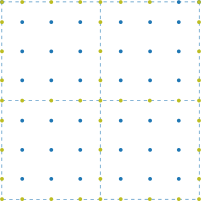
\includegraphics[width=0.48\textwidth]{../img/HighOrderBDDCMesh}\label{fig:bddc_mesh_not_decomposed}}
  \hfill
  \subfloat[Subdomain Interfaces]{\includegraphics[width=0.48\textwidth]{../img/HighOrderBDDCMeshInterface}\label{fig:bddc_mesh_interface}}\\
  \subfloat[BDDC Primal Nodes]{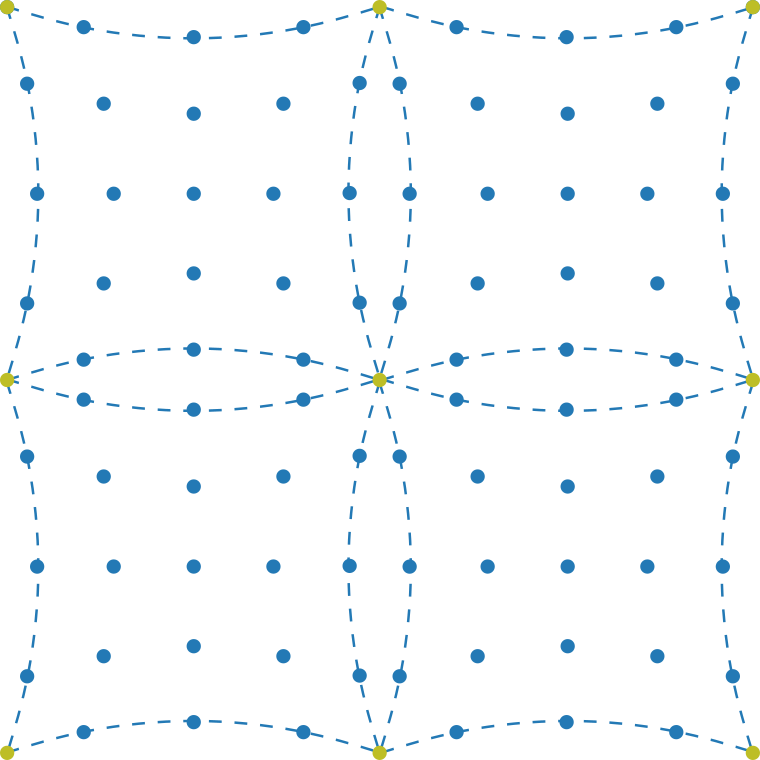
\includegraphics[width=0.48\textwidth]{../img/HighOrderBDDCMeshPrimal}\label{fig:bddc_mesh_primal}}
  \hfill
  \subfloat[BDDC Duplicated Interface Nodes]{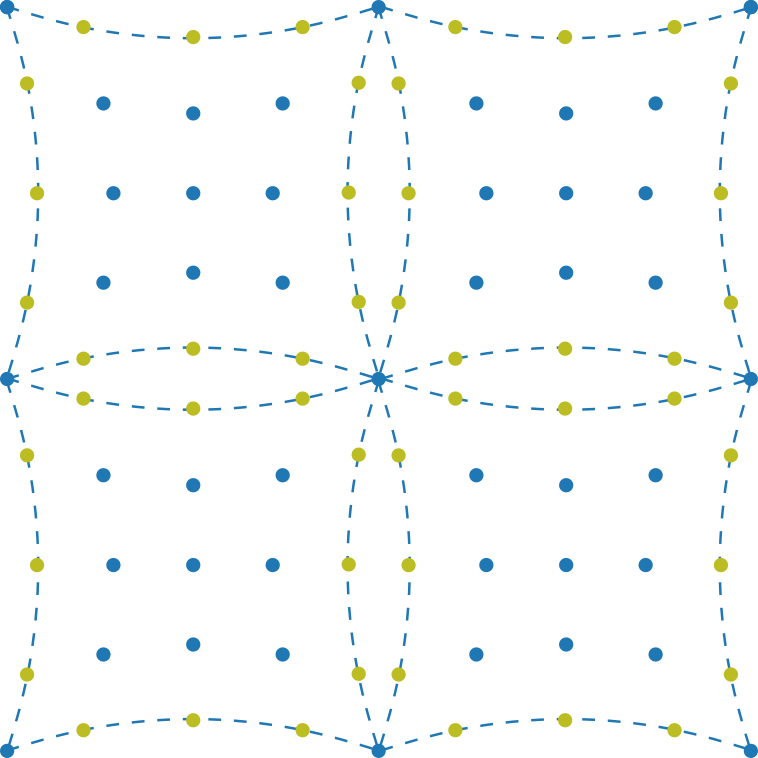
\includegraphics[width=0.48\textwidth]{../img/HighOrderBDDCMeshInterfaceBroken}\label{fig:bddc_mesh_broken_interface}}
  \caption{Non-Overlapping Decomposition of Domain for BDDC}
\end{figure}

Each subdomain problem could therefore be written as
\begin{equation}
{\color{burgundy}\mathbf{A}}^e =
\left[ \begin{array}{c c}
{\color{burgundy}\mathbf{A}}_{\text{I}, \text{I}}^e  &  {\color{burgundy}\mathbf{A}}_{\Gamma, \text{I}}^{e, T}  \\
{\color{burgundy}\mathbf{A}}_{\Gamma, \text{I}}^e    &  {\color{burgundy}\mathbf{A}}_{\Gamma, \Gamma}^e         \\
\end{array} \right]
\end{equation}
where ${\color{burgundy}\mathbf{A}}^e = {\color{blue(ncs)}\mathbf{B}}^T {\color{applegreen}\mathbf{D}} {\color{blue(ncs)}\mathbf{B}}$, as shown in Equation \ref{eq:localoperator}.

This subdomain problem can be assembled into the global problem in the typical finite element approach given by the matrix-free form in Equation \ref{eq:libceed_representation}, but in BDDC we instead create a partially subassembled problem that is easier to invert than the global problem by duplicating broken degrees of freedom along the subdomain boundaries.
Only the corner, or vertex, degrees of freedom from each element are assembled into a global coarse problem while the remaining degrees of freedom on the subdomain interfaces are duplicated in each subdomain.
The solutions on the global coarse problem and broken subdomain problems are used to construct an approximate solution to the true assembled global problem.

The coarse grid, or primal, nodes $\Pi^e$ are given by the corners of the subdomain, so we have $4$ primal nodes for each element in two dimensions and $8$ primal nodes in three dimensions.
The remainder of the subdomain we denote with an $\text{r}$.
In Figure \ref{fig:bddc_mesh_primal} the primal nodes have been highlighted.

The partially subassembled problem is therefore given by
\begin{equation}
\hat{\color{burgundy}\mathbf{A}} = \sum_{e = 1}^N \mathbf{R}^{e, T} \hat{\color{burgundy}\mathbf{A}}^e \mathbf{R}^e
\label{eq:subassembled}
\end{equation}
where
\begin{equation}
\hat{\color{burgundy}\mathbf{A}}^e =
\left[ \begin{array}{c c}
{\color{burgundy}\mathbf{A}}_{\text{r}, \text{r}}^e  &  \hat{\color{burgundy}\mathbf{A}}_{\Pi, \text{r}}^{e, T}  \\
\hat{\color{burgundy}\mathbf{A}}_{\Pi, \text{r}}^e   &  \hat{\color{burgundy}\mathbf{A}}_{\Pi, \Pi}^e            \\
\end{array} \right]
\end{equation}
and $\mathbf{R}^e$ is the subdomain injection operator. 
In this formulation, the broken degrees of freedom found on the portion of subdomain interface given by $\Gamma^e - \Pi^e$ are duplicated for each subdomain.
In Figure \ref{fig:bddc_mesh_broken_interface} the duplicated degrees of freedom across each subdomain interface have been highlighted.
This duplication reduces the amount of global communication required to solve the subassembled problem, which makes BDDC attractive as a preconditioner for high-order finite element methods.

There are BDDC formulations which enrich the primal space with edge or face averages to improve convergence.
We forgo these formulations to simplify the analysis; however these formulations can become increasingly attractive with large, high-order subdomains in three dimensions.
There is no fundamental barrier to extending the LFA of BDDC described below to formulations that use edge or face averages to improve convergence.

\begin{definition}[Balancing Domain Decomposition by Constraints Preconditioner]
The action of the BDDC preconditioner is given by
\begin{equation}
\mathbf{M}^{-1} = \mathbf{R}^T \hat{\color{burgundy}\mathbf{A}}^{-1} \mathbf{R}
\end{equation}
where $\mathbf{R}$ is the subassembly injection operator.
The inverse of the partially subassembled problem is computed by Schur complement
\begin{equation}
\hat{\color{burgundy}\mathbf{A}}^{-1} =
\left[ \begin{array}{c c}
\mathbf{I}  &  -{\color{burgundy}\mathbf{A}}_{\text{r}, \text{r}}^{-1} \hat{\color{burgundy}\mathbf{A}}_{\Pi, \text{r}}^T  \\
\mathbf{0}  &  \mathbf{I}                                                                                                  \\
\end{array} \right]
\left[ \begin{array}{c c}
{\color{burgundy}\mathbf{A}}_{\text{r}, \text{r}}^{-1}  &  \mathbf{0}                   \\
\mathbf{0}                                              &  \hat{\mathbf{S}}_{\Pi}^{-1}  \\
\end{array} \right]
\left[ \begin{array}{c c}
\mathbf{I}                                                                                                &  \mathbf{0}  \\
-\hat{\color{burgundy}\mathbf{A}}_{\Pi, \text{r}} {\color{burgundy}\mathbf{A}}_{\text{r}, \text{r}}^{-1}  &  \mathbf{I}  \\
\end{array} \right]
\end{equation}
where $\hat{\mathbf{S}}_{\Pi} = \hat{\color{burgundy}\mathbf{A}}_{\Pi, \Pi} - \hat{\color{burgundy}\mathbf{A}}_{\Pi, \text{r}} {\color{burgundy}\mathbf{A}}_{\text{r}, \text{r}}^{-1} \hat{\color{burgundy}\mathbf{A}}_{\Pi, \text{r}}^T$.
$\Pi$ denotes degrees of freedom on the assembled subdomain vertex space, while $r$ denotes degrees of freedom on the broken space given by the subdomain interior and duplicated portions of the subdomain interface.
\label{def:bddcpreconditioner}
\end{definition}

% -- Injection -----------------------------------------------------------------
\subsection{Injection Operators}
\input 05-DomainDecomposition/01-01-injection

% -- Fast Diagonalization ------------------------------------------------------
\subsection{Subdomain Solver with Fast Diagonalization}\label{sec:fdm_subdomain}
\input 05-DomainDecomposition/01-02-fastdiagonalization